\documentclass[11pt]{article}
\usepackage{array}
\usepackage{tabularx}
\usepackage{graphicx}
\usepackage{algorithm}
\usepackage{algorithmic}
\usepackage{pgfplotstable}
\usepackage{pgfplots}
\usepackage{filecontents}
\usepackage{amsmath}



\title{
	\textbf{IMS Assignment 2}
}

\author{Tobias Stahl \\ 10528199 \and Ioannis Giounous Aivalis \\ 10524851 }




\begin{document}

\maketitle


\section{Introduction}
This report is about Assignment 2 of the UvA course Intelligent Multimedia Systems. The goal of Assignment 2 is to implement functions to smooth images with a gaussian filter.\\

\section{Exercise 1}

\subsection{Excercise 1.3 - Comparison with Built-in function}
In this exercise the previously implemented functions \texttt{gaussian.m} and \texttt{gaussianConv.m} are tested and the result is compared to the matlab built-in function \texttt{fspecial('gaussian', hsize, sigma)}.

\subsection{Exercise 1.5.2 - Magnitude and orientation of different $\sigma$}
In this exercise magnitude and orientation of the picture are extracted with help of functions \texttt{gaussianDer.m}, which computes the derivative of gaussian filter G, and \texttt{gradmag.m}, which convolves the image with the derivative of the filter and returns the two images of magnitude and orientation.\\
For both the orientation and the magnitude it is clear to see, that for increasing values of $\sigma$ the smaller structures disappear and only large structures are affected by the gradient. The output of various plots are shown in Figure ~\ref{magnitude} for the magnitude and Figure for the orientation.
\begin{figure}[h!]
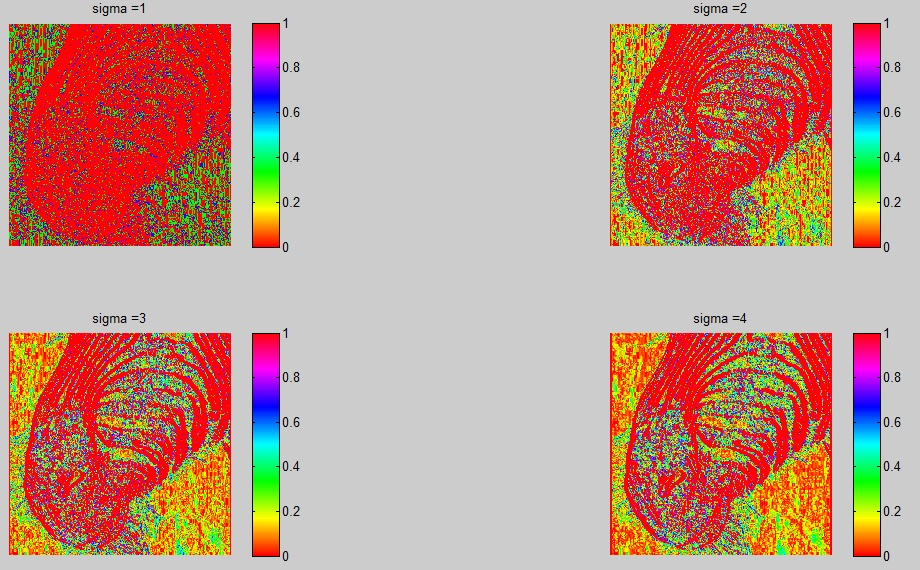
\includegraphics[scale=0.6]{Magnitude.jpg}
\caption{Magnitude of zebra.png for $\sigma = {1,2,3,4}$}
\label{magnitude}
\end{figure}

\subsection{Exercise 1.5.3 - Thresholds}
In this section pixels of the magnitude with a value below a specific threshold are set to not appear to convert the image into a binary format. Figure ~\ref{threshold} shows the output for different thresholds and $\sigma$.

\begin{figure}[h!]
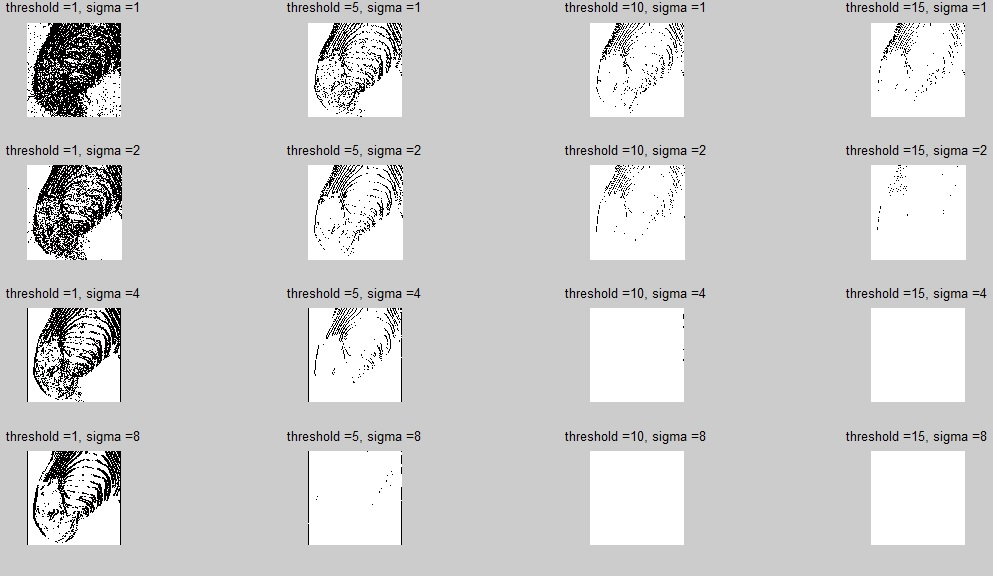
\includegraphics[scale=0.6]{thresholds.jpg}
\caption{Magnitudes after threshold filter}
\label{threshold}
\end{figure}

\subsection{Exercise 1.5.5 - Impulse}
The goal of this part is to create an impulse image and run the different filters with different $\sigma$ on that image.\\
The result image is suppose to display the filter. Figure shows the result images of this exercise.

\section{Conclusion}
In this assignment the functions to create a gaussian filter and its derivatives and to convolve those with any image were implemented and tested with different exercises. 




\end{document}